\documentclass{standalone}
\usepackage{tikz}
\usetikzlibrary{calc} % 坐标计算库
\usetikzlibrary{patterns} % 阴影填充库
\usepackage{pgfplots} % 绘图库
\usepgfplotslibrary{fillbetween} % 区域阴影
\pgfplotsset{compat=1.18} % 设置 pgfplots 版本
\usetikzlibrary{patterns.meta} % 图案库

% 常量声明
\newcommand{\xmin}{0}
\newcommand{\xmax}{3.5}
\newcommand{\ymin}{-35}
\newcommand{\ymax}{5}

\begin{document}

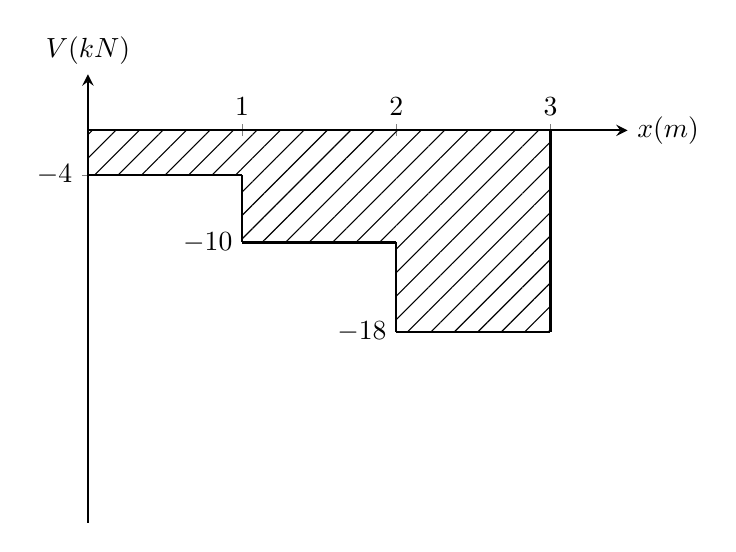
\begin{tikzpicture}
    % Shear Diagram
    \begin{axis}[
            axis lines=middle, % 学校式坐标轴
            axis line style={thick},
            xlabel={$x(m)$},
            xlabel style={right},
            ylabel={$V(kN)$},
            ylabel style={above},
            xtick={1,2,3},
            xticklabel style={anchor=south, yshift=4pt},
            ytick={-4},
            xmin=\xmin, xmax=\xmax,
            ymin=\ymin, ymax=\ymax,
            domain=0:3,
        ]
        % 定义函数和x轴
        \addplot[name path=A, domain=0:1, thick] {-4};
        \addplot[name path=B, domain=1:2, thick] {-10};
        \addplot[name path=C, domain=2:3, thick] {-18};
        \addplot[name path=AA, domain=0:1] {0};
        \addplot[name path=BB, domain=1:2] {0};
        \addplot[name path=CC, domain=2:3] {0};
        % 填充两者之间的区域
        \addplot[
            pattern={Lines[angle=45, distance=6pt]},
        ] fill between [of=A and AA];
        \addplot[
            pattern={Lines[angle=45, distance=6pt]},
        ] fill between [of=B and BB];
        \addplot[
            pattern={Lines[angle=45, distance=6pt]},
        ] fill between [of=C and CC];
        % 添加标识线或点
        \node at (axis cs:1,-10) [left] {$-10$};
        \node at (axis cs:2,-18) [left] {$-18$};
        \draw[thick] (axis cs:1,-4) -- (axis cs:1,-10);
        \draw[thick] (axis cs:2,-10) -- (axis cs:2,-18);
        \draw[thick] (axis cs:3,-18) -- (axis cs:3,0);
    \end{axis}

\end{tikzpicture}

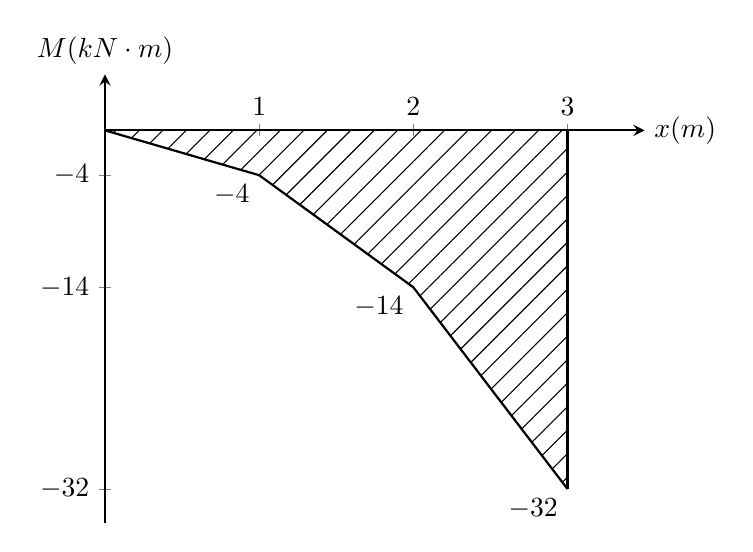
\begin{tikzpicture}
    % Moment Diagram
    \begin{axis}[
            axis lines=middle, % 学校式坐标轴
            axis line style={thick},
            xlabel={$x(m)$},
            xlabel style={right},
            ylabel={$M(kN \cdot m)$},
            ylabel style={above},
            xtick={1,2,3},
            xticklabel style={anchor=south, yshift=4pt},
            ytick={-4,-14,-32},
            xmin=\xmin, xmax=\xmax,
            ymin=\ymin, ymax=\ymax,
            domain=0:3,
        ]
        % 定义函数和x轴
        % M_1 = 5 * x
        % M_2 = M_1 + 30
        \addplot[name path=A, domain=0:1, thick] {- 4*x};
        \addplot[name path=B, domain=1:2, thick] {- 4*x - 6*(x-1)};
        \addplot[name path=C, domain=2:3, thick] {- 4*x - 6*(x-1) - 8*(x-2)};
        \addplot[name path=AA, domain=0:1] {0};
        \addplot[name path=BB, domain=1:2] {0};
        \addplot[name path=CC, domain=2:3] {0};
        % 填充两者之间的区域
        \addplot[
            pattern={Lines[angle=45, distance=6pt]},
        ] fill between [of=A and AA];
        \addplot[
            pattern={Lines[angle=45, distance=6pt]},
        ] fill between [of=B and BB];
        \addplot[
            pattern={Lines[angle=45, distance=6pt]},
        ] fill between [of=C and CC];
        % 添加标识线或点
        \draw[thick] (axis cs:3,0) -- (axis cs:3,-32);
        \node at (axis cs:1,-4) [below left] {$-4$};
        \node at (axis cs:2,-14) [below left] {$-14$};
        \node at (axis cs:3,-32) [below left] {$-32$};
    \end{axis}

\end{tikzpicture}

\end{document}